%%%%%%%%%%%%%%%%%%%%% chapter.tex %%%%%%%%%%%%%%%%%%%%%%%%%%%%%%%%%
%
% sample chapter
%
% Use this file as a template for your own input.
%
%%%%%%%%%%%%%%%%%%%%%%%% Springer-Verlag %%%%%%%%%%%%%%%%%%%%%%%%%%
%\motto{Use the template \emph{chapter.tex} to style the various elements of your chapter content.}
\chapter{Introduction}
\label{intro} 

\abstract{Each chapter should be preceded by an abstract (10--15 lines long) that summarizes the content. The abstract will appear \textit{online} at \url{www.SpringerLink.com} and be available with unrestricted access. This allows unregistered users to read the abstract as a teaser for the complete chapter. As a general rule the abstracts will not appear in the printed version of your book unless it is the style of your particular book or that of the series to which your book belongs.}

%\newline\indent
%Please use the 'starred' version of the new Springer \texttt{abstract} command for typesetting the text of the online abstracts (cf. source file of this chapter template \texttt{abstract}) and include them with the source files of your manuscript. Use the plain \texttt{abstract} command if the abstract is also to appear in the printed version of the book.}


\section{Motivations and Concepts of U-LTE}
\label{lte-motiv}

Global mobile traffic is expected to increase nearly tenfold between 2014 and 2020 due to increasing number of mobile-connected devices and the explosion of data-hungry mobile applications \cite{cisco_mobile_traffic_2015}. As visualized in Fig. \ref{figs:global-mobile-data-traffic-2015-2020}, in 2015, global mobile data traffic amounted to $3.7$ exabytes per month. In 2020, mobile data traffic worldwide is expected to reach $30.6$ exabytes per month at a compound annual growth rate of $53$ percent. Pushing traffic towards the network capacity quickly deteriorates the Quality of Services (QoSs) perceived by the users. As a result, increasing the capacity of Radio Access Networks (RANs) is one of the top-priority action plans of mobile service providers. Purchasing additional licensed spectrum is a straight-forward solution to this but radio spectrum is very much limited and expensive. Furthermore, mobile operators are at the same time challenged by the ``revenue gap'', i.e., the exponential increase in mobile traffic does not generate sufficient additional revenues required for upgrading their RANs. This circumstance has fostered the interest in cost-effective solutions to RAN capacity increase. \textit{Mobile data off-loading} and \textit{Long-Term Evolution (LTE) in unlicensed bands (U-LTE)} are among promising solutions. 

\begin{figure}[!t]
	\centering
	\includegraphics[width=0.8\columnwidth]{figures2/global-mobile-data-traffic-2015-2020.pdf}
	\caption{Global mobile data traffic from 2015-2020 \cite{cisco_mobile_traffic_2015}.}
	\label{figs:global-mobile-data-traffic-2015-2020}
\end{figure}


Mobile data offloading is the use of a complementary wireless technology to transport data originally flowing through the cellular mobile network. Wi-Fi offload and Device-to-Device (D2D) communications are the two main data offload technologies. Rules determining when and how the mobile offloading actions are triggered are set by either mobile subscribers or network operators. For the subscribers, data offloading helps them to exploit the availability of higher bandwidth data service at lower costs. For the operators, the most obvious benefit of this kind of approach is the mitigation of cellular mobile network load and thus congestion. Besides, shifting data to a complementary wireless technology leads to a number of other improvements including: the increase of the overall throughput, the reduction of content delivery time, the extension of network coverage, the increase of network availability, and better energy efficiency. Unfortunately, these benefits come with a number of challenges related to infrastructure coordination, network/technology hand-overs, service continuity, pricing, business models, and lack of standards. 

Recently, U-LTE has appeared as the most promising approach to enhance RAN capacity and address the revenue gap in mobile networks. By definition, it is an LTE technology that puts cellular signals into the unlicensed spectrum with the supports of existing LTE features including Supplemental Downlink (SDL, proposed in LTE Release 9 and later) and Carrier Aggregation (CA, proposed in LTE Release 10 and later). The original idea of LTE-U is fairly straightforward. As mentioned, mobile operators are facing a great pressure on capacity and cost. If LTE can exploit the unlicensed band (where IEEE 802.11/Wi-Fi and other radio systems are using), then it will have a considerable additional capacity at a minimal cost. U-LTE can be used to boost downlink or both uplink and downlink of LTE networks, as illustrated in Fig. \ref{figs:U-LTE-use_model}.

Historically, U-LTE was originally proposed and officially announced by Qualcomm in 2013 \cite{Qualcomm-U-LTE-2013}. Currently, it focuses on $500$ MHz of spectrum available in the $5$ GHz band. Specifically, according to the proposal from Qualcomm, U-LTE uses the U-NII-3 part of the $5$ GHz band, which has highest allowed Equivalent Isotropically Radiated Power (EIRP). While in $2.4$ GHz regulatory bodies limit EIRP to $100$ mW (in Europe) or $200$ mW (in United States), the U-NII-3 enjoys the rights to go as high as $1000$ mW outdoors.

\section{Benefits and Obstacles of U-LTE}
\label{lte-ben}

U-LTE is expected to offer numerous benefits to mobile network operators, service providers, and consumers. \textit{First}, free unlicensed spectrum provides additional capacity to the network at a minimal cost. Therefore, U-LTE appears to be a very inexpensive way to meet the future traffic growth. \textit{Second}, U-LTE will give operators the option to make use of unlicensed spectrum with a unified network, offering potential operational cost saving, improving spectral efficiency, and providing a better user experience. Compared to the Wi-Fi offloading technology, U-LTE has the potential to offer significantly better coverage and higher spectral efficiency while allowing seamless flow of data across licensed and unlicensed in a single core network. \textit{Third}, U-LTE could also take advantage of the robust security features of LTE networks. \textit{Finally}, while Wi-Fi offloading leads to less traffic on mobile networks and thus may result in revenue losses in data services, U-LTE could represent an incremental ability on mobile service providers to directly bill for data usage.

\begin{figure}[!t]
	\centering
	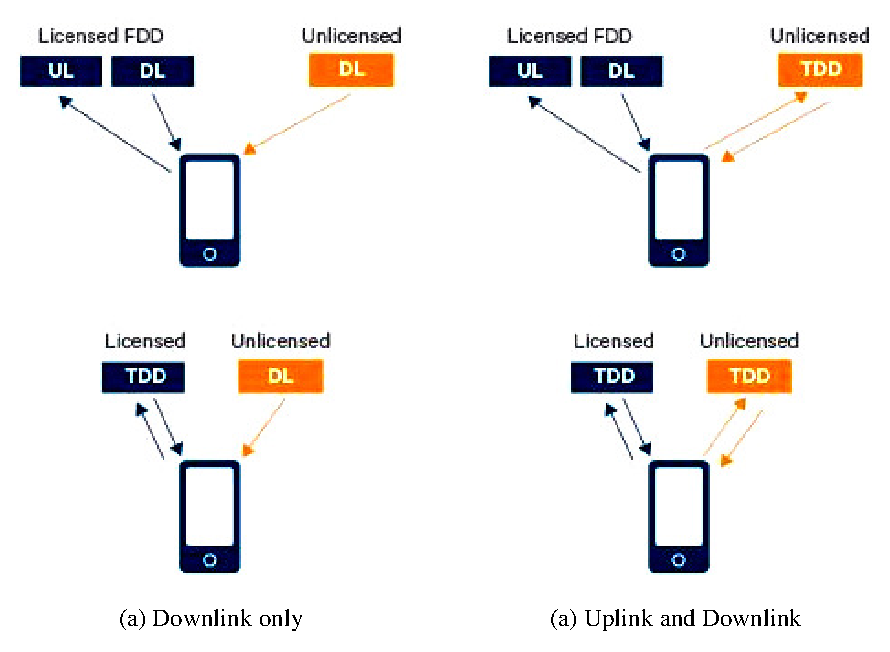
\includegraphics[width=0.7\columnwidth]{figures2/U-LTE-use_model}
	\caption{Use cases of U-LTE.}
	\label{figs:U-LTE-use_model}
\end{figure}

U-LTE is also facing a number of substantial obstacles. \textit{First}, even though U-LTE is not charged for the use of unlicensed spectrums, compared to Wi-Fi, its network deployment could be more expensive. LTE chipset itself is several times more expensive than that of Wi-Fi (a few tens of dollars compared to a few dollars or less than one dollar). LTE base stations and other network devices are likely to cost substantially more. Also, LTE operators need to deploy and maintain expensive back-haul links. \textit{Next}, U-LTE will work only with LTE-capable devices while there have been many more devices that feature Wi-Fi connectivity than LTE. Wi-Fi is nearly always integrated with laptops, tablets, cameras, and other connected consumer devices. \textit{Additionally}, from technical perspectives, the premium features provided by U-LTE (e.g., seamless voice and data roaming) may not prove sufficiently more valuable than those offered by emerging Wi-Fi technologies such as Hotspot 2.0, so-called Wi-Fi Certified Passpoint, which is a new standard for public-access Wi-Fi that enables seamless roaming among Wi-Fi networks and between Wi-Fi and cellular networks. \textit{Finally}, the biggest challenge of U-LTE is its coexistence with other radio networks operating in the same frequency bands. This challenge will be studied in subsequent sections.

\section{Three Types of U-LTE}
\label{lte-types}
U-LTE comprises of three different flavors: LTE unlicensed (LTE-U), Licensed Assisted Access LTE (LAA-LTE), and MuLTEfire. The first two flavors require ``anchoring licensed spectrum'', i.e., they operate primarily in licensed spectrum and opportunistically exploit unlicensed spectrum for an additional bandwidth boost. Devices are still anchored in licensed spectrum for LTE management/control signaling and high QoS data while using the unlicensed spectrum for only best-effort or delay-tolerant data. The third flavor is developed by Qualcomm and requires no licensed spectrum at all, therefore, it is often referred to as ``standalone'' U-LTE. MuLTEfire is designed for indoor use and deployments by enterprises, cable companies and other service providers without ownership of expensive bandwidth licenses. However, at present time, there are very few technical details available about MuLTEfire.


%TODO: The remainder of this section was previously its own chapter, but appears to fit best in this section 
\subsection{LTE-U}

\noindent This is the simplest form of U-LTE that requires minor modifications in LTE protocol stack. Therefore, it can quickly facilitate pre-standard equipment manufacturing and deployment. LTE-U first attempts to select clear channel to access. If no clear channel is found, it will employs Carrier-Sensing Adaptive Transmission (CSAT) which is a Time-Division Multiplex (TDM) coexistence based on medium sensing. CSAT employs ``duty-cycling'' instead of LBT mechanism. Compared to LBT or CSMA, the small cell senses the medium for a longer duration (around $10$s of millisecond to $200$ millisecond) and according to the observed medium activities, the algorithm gates off LTE transmission proportionally. In particular, CSAT defines a time cycle where the small cell transmits in a fraction of the cycle and gates off in the remaining duration. The duty cycle of transmission versus gating off is dictated by the sensed medium activity of neighboring RANs. The TDM cycle can be set to a few tens or hundreds of millisecond, which can effectively accommodate the activation/de-activation procedures while controlling the data transmission delay. CSAT is illustrated in Fig. \ref{figs:LTE-U}. An important observation from Fig. \ref{figs:LTE-U} is that during the LTE ``on'' period, Wi-Fi is blocked by LTE-U transmissions. During the LTE ``off'' period, Wi-Fi will detect that the channel is free and can schedule its transmissions following its CSMA-CA protocol.

LTE-U is only applicable in areas where there are no strict LBT requirements for operations in unlicensed bands (e.g., US. Korea, China). It is a non-standard version of U-LTE, being developed outside of the 3GPP standards process. LTE-U is supported by LTE-U Forum formed in 2014 by Verizon in cooperation with Alcatel-Lucent, Ericsson, Qualcomm Technologies Inc. (a subsidiary of Qualcomm Incorporated), and Samsung.

\begin{figure}[!t]
	\centering
	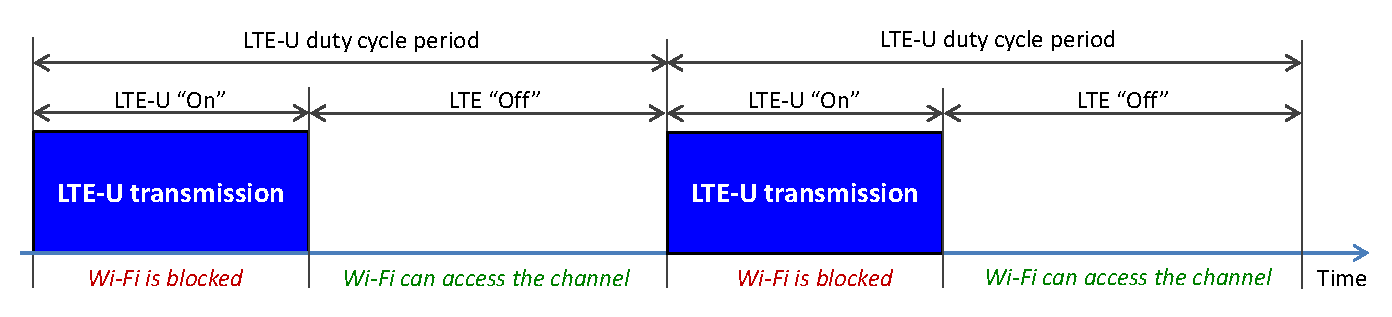
\includegraphics[width=0.95\columnwidth]{figures2/LTE-U}
	\caption{Duty-cycling mechanism employed by LTE-U.}
	\label{figs:LTE-U}
\end{figure}

\subsection{LAA-LTE}

\noindent In many areas such as Europe, Japan and India, there exist regulations for unlicensed spectrum that require equipment to periodically check for presence of other occupants in the channel, so-called LBT, in millisecond scale. LAA-LTE is designed for use in those areas or for global use. It requires a number of modifications so that LTE transmissions can meet regulatory requirements in LBT regions. Similar to LTE-U, LAA-LTE first tries to choose the cleanest channel based on Wi-Fi and LTE measurements to operate on. In the event that no clean channel is available, LBT algorithm is used to compete the medium with other RANs in the same channel. For LBT, FBE- and LBE-based mechanisms specified in \cite{LBT-ETSI-2014} have been used. Details of these two mechanisms have been presented in section \ref{subsec:ETSI-LBT-overview}.

Assuming that LBE-based LBT is employed for LAA-LTE. Before transmission, CCA using ED is performed. If the channel is clear during a CCA slot ($20$ microseconds or longer), transmission is started immediately. Otherwise, ECCA is performed. If the channel is clear during $N$ CCA slots, transmission is started immediately. $N$ is a random integer uniformly distributed from $1$ to $q$, where $q \in \{4,5,...,32\}$. The total time to occupy the channel without CCA is limited by $(13/32)q$ milliseconds (e.g., $13$ milliseconds when $q$ is $32$). Two simplified scenarios with LAA-LTE (employing LBE-based LBT) and Wi-Fi systems operating in the same channel are illustrated in Fig. \ref{figs:LAA-LTE}. In the first scenario, the LAA-LTE system, upon having data frames to send, performs CCA and then ECCA (with $N=7$) since there is an ongoing Wi-Fi transmission. The ECCA procedure is frozen and then resumed when another Wi-Fi transmission takes place and then completes, respectively. The LAA-LTE system finally transmits its frames once ECCA counter $N$ reaches zero. In the second scenario, the Wi-Fi system, upon having data frames to send, performs CCA and then back-off procedure (with $\mathrm{BI_{slots}} = 7$) since there is an ongoing LAA-LTE transmission. The back-off procedure is frozen and resumed when another LAA-LTE transmission takes place. The Wi-Fi system finally transmits its frames once back-off counter $w$ reaches zero.

LTE was originally designed for licensed spectrum and a centralized management (i.e., network-controlled) model, it is generally an ``always-on'' technology. As a result, adapting to LBT is a marked change for the LTE protocol. Compared to LTE-U which is downlink-only in unlicensed bands, LAA-LTE may allow bi-directional traffic in unlicensed bands.

LAA-LTE is currently actively supported by 3GPP and will be included in 3GPP LTE Release 13 (to be published by March 2016). T-Mobile USA and Verizon Wireless have indicated their interests in deploying pre-standard LAA-LTE systems for evaluations and commercial services in 2016.

\begin{figure}[!t]
	\centering
	\includegraphics[width=0.9\columnwidth]{figures2/LAA-LTE}
	\caption{CCA and ECCA mechanisms employed by LAA-LTE.}
	\label{figs:LAA-LTE}
\end{figure}

\subsection{MuLTEfire}

%TODO: The section below was previously in the open research questions section, but the corresponding subsection was not in the TOC submitted to springer
At this time there are very few technical details available about MuLTEfire. It is unknown which MAC protocols or coexistence mechanisms are employed in this type of U-LTE. Also, since licensed frequency is not used for LTE network management and control signaling, as opposed to the conventional LTE and the other two variants of U-LTE (i.e., LTE-U and LAA-LTE) that are license anchored, MuLTEfire may lose all advantages of native LTE technologies. It is expected that MuLTEfire will be less efficient than LTE-U and LAA-LTE and therefore its achievable performance/efficiency may be just marginally better than that of Wi-Fi. Then the question on the applicability of MuLTEfire needs to be answered.


\section{Coexistence of U-LTE and Wi-Fi}
\label{coexist}

It is well known that multiple radio communications technologies operating in a common frequency band will negatively affect each other if respectful coexistence mechanisms are not employed. As a result, despite the fact that U-LTE can offer various benefits as mentioned before, its coexistence with Wi-Fi and other radio systems that operate in the $5$ GHz frequency band is the biggest concerns. In details, it has been believed that U-LTE may considerably interfere Wi-Fi systems and/or grasp more radio resources when they are operating in the same frequency band due to the following facts.

\textit{First}, LTE was originally designed to work in its own licensed band rather than to coexist with Wi-Fi in a shared band. LTE employs Orthogonal Frequency-Division Multiple Access (OFDMA) and transmits almost continuously without any mechanism for spectrum sharing. Wi-Fi, on the other hand, employs Listen Before Talk (LBT) MAC with a few key additional features that go beyond LBT requirements specified by European Telecommunications Standards Institute (ETSI) \cite{LBT-ETSI-2014}. As a result, U-LTE might overwhelm Wi-Fi neighbors with its aggressive transmissions if no relevant coexistence measure is implemented.

\textit{Second}, the typical lengths of each transmission of these two technologies are not the same. LTE, due to its basic protocol design and scheduled nature, generally transmits long frames (i.e., multiple ms), whereas a large percentage of Wi-Fi frames are sub-millisecond in duration. For this reason, equitable access to the medium, evaluated in terms of how often a technology is able to start a transmission, does not necessarily translate into equitable airtime.

\textit{Third}, a license-anchored system (LTE-U or LAA-LTE) operates simultaneously in licensed and unlicensed bands and thus can dynamically move traffic between the bands on a granular basis (e.g., per-user and per-flow). As a result, such a system is inherently less sensitive to collisions and congestion in the unlicensed bands than is a system operating solely in unlicensed spectrum. This may reduce the incentive for a license-anchored system to develop effective coexistence mechanisms in the unlicensed band.

In fact, U-LTE is still a nascent LTE technology with many technical details to be determined. Proponents of U-LTE include Qualcomm, Ericsson, Alcatel-Lucent, Huawei, LTE-U Forum, 3rd Generation Partnership Project (3GPP), Verizon Wireless, T-Mobile US, etc. At the same time, CableLabs, Google, Wi-Fi Alliance, The Institute of Electrical and Electronics Engineers Standards Association (IEEE-SA) and many Wi-Fi interested companies are participating in and following closely the development of U-LTE technology. They have been expressing their concern on a critical need for strong coexistence between U-LTE and Wi-Fi to ensure responsible and fair use of unlicensed spectrum. As a result, various studies on the coexistence of U-LTE and Wi-Fi have been carried out by both industry and academia. Besides, a number of reports and comments related to this concern have been filed with the Federal Communications Commission (FCC).


\section{Requirements of U-LTE Coexistence Mechanisms}
\label{reqs}

Even though the unlicensed bands may be used by anyone, there is a series of government guidelines and regulations to be followed. Those guidelines and regulations aim to ensure that different radio systems that operate in the same frequency bands are good neighbors of each other.

In particular, for coexistence with Wi-Fi, at least U-LTE must satisfy local regulations such as the maximum transmission power in specific bands and the avoidance of bands dedicated to protected services. Furthermore, an U-LTE system should not cause any higher interference to a neighboring Wi-Fi system than a typical Wi-Fi system operating on the same channel. In other words, the impact of a U-LTE device to Wi-Fi devices (in terms of collision rate and probability of successful channel access) should be similar to that caused by a typical Wi-Fi device. These requirements ask for inclusions of a number of new features in LTE. For example, U-LTE should select a carrier which is least occupied in the area and it should dynamically change operating frequency to avoid conflict with protected systems, such as radar. It should also apply LBT or Clear Channel Assessment (CCA) techniques to check that a channel is free before making a transmission. Exactly how these decisions are made will be key aspects of U-LTE system designs.

%%%%%%%%%%%%%%%%%%%%%%%% referenc.tex %%%%%%%%%%%%%%%%%%%%%%%%%%%%%%
% sample references
% %
% Use this file as a template for your own input.
%
%%%%%%%%%%%%%%%%%%%%%%%% Springer-Verlag %%%%%%%%%%%%%%%%%%%%%%%%%%
%%
%% BibTeX users please use
%% \bibliographystyle{}
%% \bibliography{}

\begin{thebibliography}{99.}%
\bibitem{cisco_mobile_traffic_2015}``Cisco visual networking index: Global mobile data traffic forecast update 2014-2019,'' white paper, Cisco, 2015.	
	
\bibitem{Qualcomm-U-LTE-2013}``Extending {LTE} advanced to unlicensed spectrum,'' white paper, Qualcomm Inc., Dec. 2013.

\bibitem{LBT-ETSI-2014} \emph{ETSI EN 301 893 V1.7.2 (2014-07): Broadband radio access networks (BRAN);	5 GHz high performance RLAN; Harmonized EN covering the essential requirements of article 3.2 of the R\&TTE Directive}, European Telecommunications Standards Institute Std., 2014.	
\end{thebibliography}
